%Use one of the two documentclass lines depending on aspect ratio needed
% for 4x3 aspect ratio slides
%\documentclass{beamer}
%for 16x9 (modern wide screen) aspect ratio slides
\documentclass[aspectratio=169]{beamer}
\usepackage{breqn}
\usepackage{mathtools}
\usepackage[authordate,bibencoding=auto,strict,backend=biber,natbib]{biblatex-chicago}
\addbibresource{references.bib}
\usepackage{bm}

\usepackage{tikz}
\usepackage{tikz-3dplot}
\usetikzlibrary{positioning, fit, shapes, arrows.meta}
\usepackage{subfigure}

\usepackage{etoolbox} % for \ifnumcomp
\usepackage{listofitems} % for \readlist to create arrays

\tikzset{>=latex} % for LaTeX arrow head
\colorlet{myred}{red!80!black}
\colorlet{myblue}{blue!80!black}
\colorlet{mygreen}{green!60!black}
\colorlet{mydarkred}{myred!40!black}
\colorlet{mydarkblue}{myblue!40!black}
\colorlet{mydarkgreen}{mygreen!40!black}
\tikzstyle{node}=[very thick,circle,draw=myblue,minimum size=22,inner sep=0.5,outer sep=0.6]
\tikzstyle{connect}=[->,thick,mydarkblue,shorten >=1]
\tikzset{ % node styles, numbered for easy mapping with \nstyle
  node 1/.style={node,mydarkgreen,draw=mygreen,fill=mygreen!25},
  node 2/.style={node,mydarkblue,draw=myblue,fill=myblue!20},
  node 3/.style={node,mydarkred,draw=myred,fill=myred!20},
}
\def\nstyle{int(\lay<\Nnodlen?min(2,\lay):3)} % map layer number onto 1, 2, or 3


\tdplotsetmaincoords{60}{-20}
\renewcommand{\P}{\mathcal{P}}
% Oxford Maths theming
\usetheme{oxfordmaths}

% \newtheorem{theorem}{Theorema}
% \newtheorem{lemma}[theorem]{Lemma}
% \newtheorem{corollary}[theorem]{Corollarium}
\newtheorem{prop}{Proposition}

% Set author etc info
\title[A Geometric Approach to Quantum Circuit Complexity] %short version of title for slide footer
{A Geometric Approach to Quantum Circuit Complexity} %full title for titlepage
\author{Yuhao Han}
\institute{Mathematical Institute\\University of Oxford}
\date[\today]  %short date for slide footer
{} %main date for title page,
                        %can overload it to show say 'Conference X, Date Y'


%% Now for the actual slides %%
\begin{document}

\begin{frame}[plain]
  \titlepage
\end{frame}


\begin{frame}
	\frametitle{Complexity of Quantum Circuits}

	\begin{itemize}
		\item A quantum computation is usually described as a sequence of logical gates, each only acting on a few qubits.
		\item These gates are unitary operators on the state space of the qubits.
		\item The difficulty of performing a unitary operation is characterized by the minimal number of gates required to implement it.
		\item \emph{Given a unitary operator $U$, what is the minimal number of gates required to implement it?} This is the central problem in quantum circuit complexity.
	\end{itemize}
\end{frame}

\begin{frame}[allowframebreaks]
	\frametitle{A Geometric Approach \citep{Nielsen2006}}

\begin{itemize}
		\item Given an operator $U \in SU(2^n)$ generated by Hamiltonian $H(t)$ satisfying the Schrödinger equation.
			$H(t)$ has a Pauli operator expansion $H = \sum_{\sigma}h_{\sigma}\sigma + \sum_{\tau}h_{\tau}\tau$, where $\sigma$ are one and two body interactions, $\tau$ are other interactions, with the coefficients $h_{\sigma}, h_{\tau} $ in real numbers.
		\item  Define a cost function as
$$
F(H) = \sqrt{\sum_{\sigma} h_{\sigma}^2 + p^2\sum_{\tau}h_{\tau}^2}
$$
\item The length of the path, $U(t): [0, t_f] \rightarrow SU(2^n)$ connecting $I$ and $U$ is defined as 
$$
d([U]) := \int_0^{t_f} dt F(H(t))
$$
\item $F(H)$ can be regarded as the norm associated with the metric on $SU(2^n)$ whose components are
$$
	g_{\sigma \tau} = \begin{cases}
		0 \text{ if } \sigma \neq \tau \\
		1 \text{ if } \sigma  = \tau \text{ is one or two-body interactions} \\
		p^2 \text{ otherwise ($p$ is an arbitrary penalty)}
	\end{cases}
$$
\item Let $d(I, U)$ denote the length of the minimal geodesic connecting $I$ and $U$. 
\item \textbf{Claim 1}. $d(I, U)$ gives a lower bound on the number of 1- or 2- body gates to exactly generate $U$ \citep{nielsen2005}.	
\item \textbf{Claim 2}. Up to a polynomial factor, $d(I, U)$ gives the number of one- or two-body gates required to approximate $U$ for any precision \citep{Nielsen2006}.
\end{itemize}
\end{frame}

\begin{frame}[allowframebreaks]
	\frametitle{Nielsen's Approach in Three Steps}
Overall idea: corresponding unitary of the modified Hamiltonian is close to the original. 

\begin{itemize}
\item Let $H(t)$ be time-dependent Hamiltonian generating $U$ over time interval $[0, t_f]$.
Let $H_p(t)$ be the projected Hamiltonian obtained by removing all three- or more-body terms, and $U_p$ be its corresponding unitary operator.
$||U- U_p|| \leq \frac{d(I, U)}{2^n}$.
\item Divide the time interval $[0, t_f]$ into $N$ small steps, and calculate the mean Hamiltonian $\bar{H}_i$ over each small interval. (The mean Hamiltonian over an interval is defined as $\frac{1}{a-b} \int_b^a H(t)dt$) 
Denote the corresponding unitary as $U_{M, i}$. 
We can show that $U_{M, i}$ is close to $U_{P, i}$, where $U_{P, i}$ is the unitary generated by the original Hamiltonian on the $i$-th interval.
\item The unitary $U_{M, i}$ has a time independent Hamiltonian consisting of only one- or two-body interactions. 
So $U_{M, i}$ can be approximated by a reasonable number of one- or two-body gates with arbitrary precision.
\item Concatenation of the each $U_{M, i}$ gives $U_{M}$, which is a good approximation to $U$ and can be generated by a reasonable number of one- and two-body gates.
\end{itemize}
\begin{theorem}
For any unitary $U$ acting on $n$ qubits, we can use $O(n^6 d(I, U)^3)$ one- and two-qubit gates to approximate it with arbitrary precision.
\end{theorem}
\end{frame}

\begin{frame}
	\frametitle{A Demonstration}
	\begin{figure}[htbp]
		\centering
		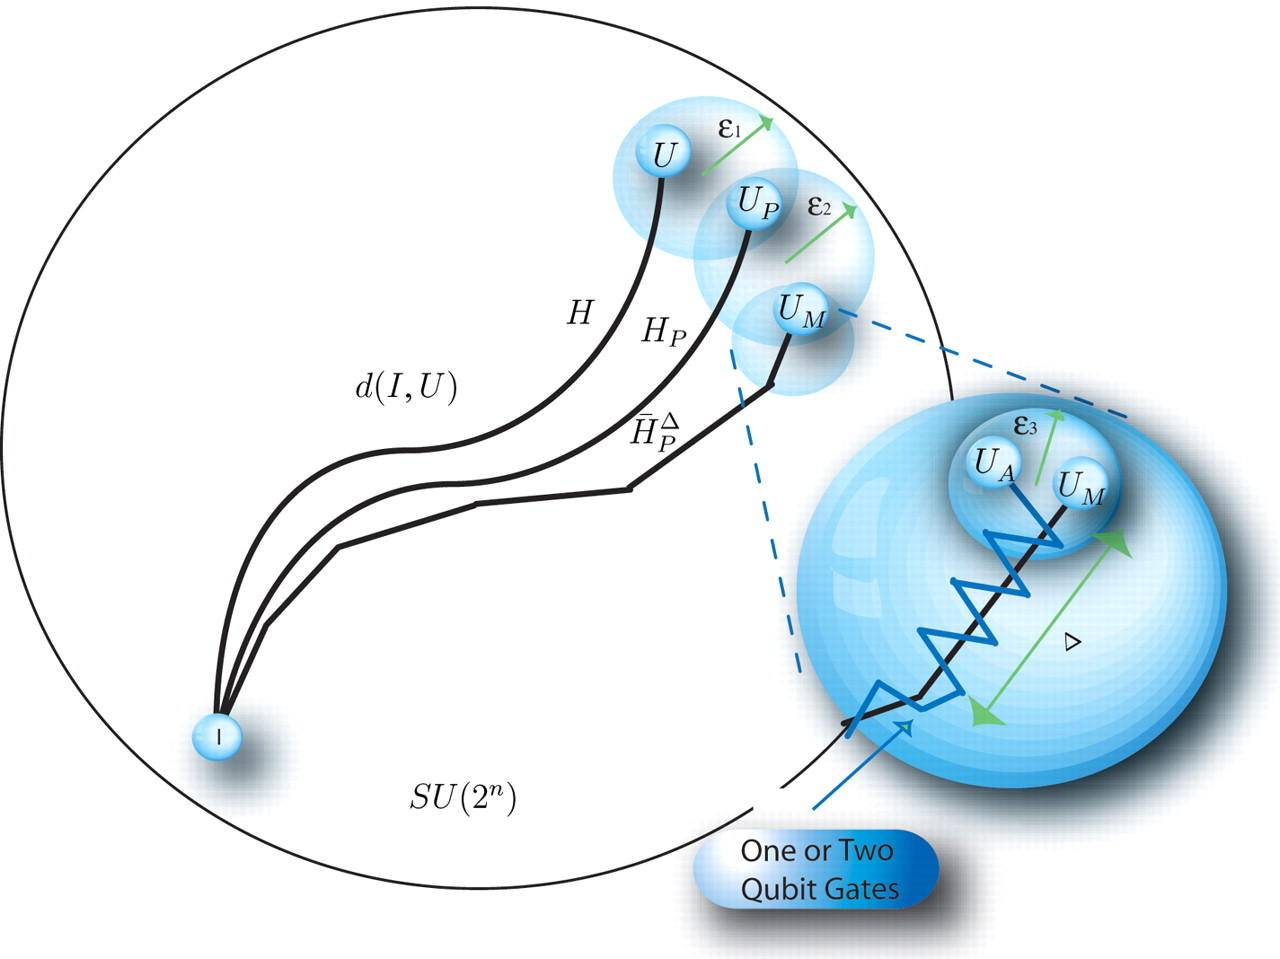
\includegraphics[width=0.5\textwidth]{demo.jpg}
		\caption{Demonstration of the Three Step Approximation \citep{Nielsen2006}}
		\label{fig:Demonstration of the Three Step Approximation}
	\end{figure}
\end{frame}

\begin{frame}
	\frametitle{Expand the Geometric Theory: Finding the Geodesic}	
	Nielsen's theory allow us to use powerful tools in geometry to study quantum circuits. 

	Finding the minimal geodesic, however, is hard (classically intractible).
	\begin{itemize}
		\item Find the geodesic on a reduction of $SU(2^n)$.
		\begin{itemize}
			\item Quotient by Clifford group.
			\item Quotient by Permutation group. Inspired by permutation invariant quantum circuit \citep{mansky2023permutationinvariantquantumcircuits}
			\item Study particular circuits such as those related to Quantum fourier transform.
		\end{itemize}
	\end{itemize}

	\textbf{Methodology}. 
	\begin{itemize}
		\item Designing new metrics that are homogeneous and right-invariant.
		\item Exploit the rich mathematical structure. Lie Theory, Topology, Differential Geometry, etc 
		\item Computer simulations.
	\end{itemize}
\end{frame}

\begin{frame}
	\frametitle{Further Direction}
	\begin{itemize}
		\item Given a minimal geodesic, can we construct the minimal circuit to generate any unitary operation? 
		\begin{itemize}
			\item Nielsen method is constructive, but does not guarantee the minimality
		\end{itemize}
		\item Extend the results to other sets of universal gates.
		\begin{itemize}
			\item fault-tolerant codes.
		\end{itemize}
	\end{itemize}
	From a wider perspective. What will
	Interaction with Clifford group: will it show insights to the origin of quantum supremacy?
\end{frame}

\begin{frame}
	\frametitle{The End}
	Thank you for listening!
\end{frame}

\begin{frame}[allowframebreaks]
	\frametitle{References}
	\printbibliography
\end{frame}

\begin{frame}[allowframebreaks]
	\frametitle{The Pauli Geodesic}

To find geodesic is to solve the geodesic equation
$$
	\frac{d}{dt}\left(\frac{\partial F}{\partial y^j}\right) = \frac{\partial F}{\partial x^j}
$$

We choose Pauli coordinates as the local coordinate, whose value corresponding to some unitary is given by 
$$
x^{\sigma}:= \frac{i \cdot \text{tr}(\text{ln}(U)\sigma)}{2^n}
$$ 

One class of geodesic arises from isometry of Pauli group is the Pauli geodesic in the form of 
$$
U(t) = e^{-i H t}
$$
where $H$ is a Hermitian matrix.

Nielsen showed that finding the minimal Pauli geodesic is equivalent to closest vector in lattice problem.

\begin{theorem}
If the minimal geodesic between $U$ and $I$ is unique, it must be a Pauli geodesic.
\end{theorem}
\begin{theorem}
There exists exponentially long minimal Pauli geodesic.
\end{theorem}
\end{frame}


\begin{frame}[allowframebreaks]
\frametitle{Nielsen's Three Lemma}

\textbf{Lemma 1.}
Let $H_p(t)$ be the projected Hamiltonian obtained from $H(t)$ by removing all the three- or more-body terms. Let $U_p$ be its corresponding unitary operator. 
We have 
$$
	||U - U_p|| \leq \frac{2^n d(I, U)}{p}
$$
Choosing $p = 4^n$, it gives $||U - U_p || \leq \frac{d(I, U)}{2^n}$ .

\textbf{Lemma 2}.
Let $U$ be generated by $H(t)$ over time interval $[0, \Delta]$ such that $||H(t)|| \leq c$.
Define the mean Hamiltonian $\bar{H} = \frac{1}{\Delta} \int_0^{\Delta} H(t) dt$. 
Then 
$$
	||U - e^{-i\bar{H}\Delta}|| \leq O(c^2 \Delta^2)
$$
\textbf{Lemma 3}.
Suppose $H$ is a time-independent Hamiltonian on $n$-qubits containing only one- and two-body interactions, and $|h_{\sigma}| \leq 1$.
Then there exists a unitary $U_m$ such that
$$	||e^{-iH\Delta} - U_m|| <  O(n^4 \Delta^3)$$
and $U_m$ can be generated by at most $O(n^2/\Delta)$ one- and two-body gates.

\end{frame}
\end{document}
